
\documentclass[journal]{IEEEtran}


\usepackage [utf8] {inputenc}
\usepackage [english] {babel}
\usepackage [final] {microtype}
\usepackage {amssymb}
\usepackage {amsmath}
\usepackage {amsfonts}
\usepackage {graphicx}
\usepackage {dblfloatfix}
\usepackage {csquotes}
\usepackage {mathtools}
\usepackage {float}
\usepackage {hyperref}
\usepackage {listingsutf8}
\usepackage{chngcntr}

\renewcommand {\a} {\alpha}
\renewcommand {\b} {\beta}
\newcommand {\g} {\gamma}
\newcommand {\G} {\Gamma}
\newcommand {\h} {\eta}
\renewcommand {\d} {\delta}
\newcommand {\e} {\varepsilon}
\newcommand {\f} {\varphi}
\renewcommand {\l} {\lambda}
\newcommand {\s} {\sigma}
\renewcommand {\i} {\iota}
\renewcommand {\th} {\vartheta}
\newcommand {\z} {\zeta}
\renewcommand {\O} {\Omega}
\renewcommand {\o} {\omega}
\newcommand {\D} {\cdot}
\newcommand {\Adj} {\dagger}
\newcommand {\Tr} {\intercal}

\newcommand {\m} [1] {\( #1 \)}
\newcommand {\V} [1] {\underline {#1}}
\newcommand {\M} [1] {\underline {\underline {#1}}}
\newcommand {\T} [1] {\tilde {#1}}
\newcommand {\RB} [1] {\left( #1 \right)}
\newcommand {\SB} [1] {\left[ #1 \right]}
\newcommand {\CB} [1] {\left\{ #1 \right\}}
\newcommand {\DB} [1] {\left[ \! \left[ #1 \right] \! \right]}
\newcommand {\Fl} [1] {\left \lfloor #1 \right \rfloor}
\newcommand {\Cl} [1] {\left \lfloor #1 \right \rfloor}
\newcommand {\Nm} [1] {\left \vert #1 \right \vert}
\newcommand {\VNm} [1] {\left \Vert #1 \right \Vert}
\newcommand {\R} [1] {\sqrt {#1}}
\newcommand {\Min} [1] {\underset {#1} {\mathrm {min}}\;}
\newcommand {\IP} [1] {\left \langle #1 \right \rangle}
\newcommand {\Stack} [1] {\startsubstack #1 \stopsubstack}
\newcommand {\Disp} [1] {
   \begin {align*}
      #1
   \end {align*}
}


\begin{document}

\title{Dantzig Selector Applied on mm-Wave MIMO Channel Estimation and and Error Analysis}

\author{Tzu-Yu Jeng \\
        Hsuan-Jung Su%
\thanks{Hsuan-Jung Su is with the Department
of Electrical Engineering, National Taiwan University.}
\thanks{Manuscript received April 1, 2020; revised April 1, 2021.}}

\markboth{IEEE Journal of whatever,~Vol.~0, No.~0, June~2020}%
{Jeng and Su: Dantzig Selector Applied on mm-Wave MIMO Channel Estimation}



\maketitle

\begin{abstract}
Multiple-input multiple-output communication systems in the millimeter-wave band are gradually being adopted.
A larger antennae array makes channel estimation more difficult.
Meanwhile, hybrid beamforming, which utilizes fewer RF chains, is applied too, so that new estimation methods have to be designed.
This can be seen as a compressive sensing problem, for which Orthogonal Matching Pursuit is usually used.

We consider a single user, hybrid structure with a uniform linear array with both precoders and combiners on each side.
We generate random beamforming matrices and use Dantzig Selector to estimate the channel in the space frequency domain.
Then, we give a quantitative bound (which holds for high probability) on the expected error norm.
To reduce the complexity, we cast it as a linear program, and suggest the basis pursuit denoising form.
Numerical results show that DS gives a superb regularization, especially when the sample is less sufficient and the noise level is higher.
We therefore propose that DS may be used, when the number of RF chains is more limited or when fewer stages of estimation are possible.
\end{abstract}

\begin{IEEEkeywords}
channel estimation, compressive sensing, sparsity, Dantzig Selector, regularization, restricted isometry
\end{IEEEkeywords}

\begin {figure*} [!b]
\centering
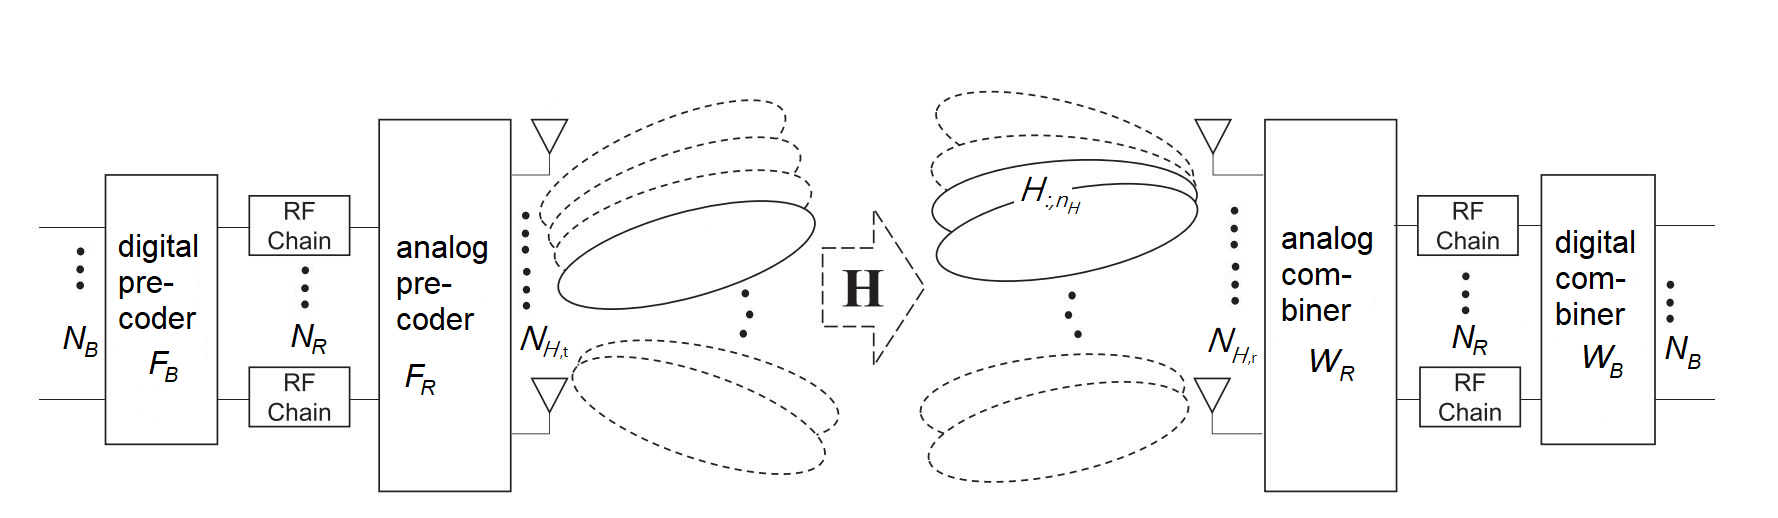
\includegraphics [width = \textwidth] {system.png}
\caption {Schematic diagram of the hybrid beamforming system we consider.}
\end {figure*}

\section{Introduction}

\subsection {Background}

Multiple-input multiple-output (MIMO) communication systems will be part of the 5G specification.
With a large number of antennae on both transmitter and receiver ends, MIMO is expected to provide a large signal gain.
Parallel and redundant transmission of data improves the error-correcting ability, and beamforming improves the signal level.
The millimeter wave (mm-wave) is adopted, since its smaller wavelength (and thus higher frequency) makes wider bands available.
Moreover the antennae may be closer-spaced, allowing us to increase their number \cite {RSM13}.
However, because of a larger antennae array and of larger noise corruption in higher frequency, estimation of MIMO channel state information gives rise to higher complexity, and hence higher hardware overhead and power consumption.
Indeed, RF chains are more expensive and power-consuming, so there is growing attention on hybrid beamforming, where there are not fewer RF chain than the antennae.

If we consider a slow varying MIMO channel for simplicity, in terms of a channel representation, to estimate the channel is to determine the parameters of the representation.
It amounts to invert a linear system whose dimension is the number of antennae, for which conventional training-based algorithms are not very effective.
Fortunately, physical evidence has suggested that mm-wave channel are poor in scattering \cite {ALS14}, which reduces the number of paths, and compressive sensing techniques may be used.
Generally speaking, compressive sensing aims to reconstruct an underdetermined linear system, when the sparsity of solution guarantees successful recovery for most cases.
In our settings for hybrid beamforming structure, a way of generating the sensing matrix and pilot vectors in the estimation stage has to be devised and justified.

\subsection {Literature}

Compressive sensing approaches can be divided into two categories, the convex programming approach and the greedy approach \cite {RDD18}.
We will discuss one from each in more detail: Dantzig Selector and Orthogonal Matching Pursuit.
For the the convex programming approach, Dantzig Selector (DS) is one of the earlier method, and it recovers the sparse signal with expected error norm bounded with overwhelming probability, and near optimality \cite {CaT07}.
DS is an minimization problem on \m {\ell_1}-norm, with \m {\ell_\infty}-constraint, which may be recast as a linear program, so that techniques from convex optimization may be used.
For our purpose in MIMO channel estimation, physical evidences suggest that mm-wave channels are sparse in the number of paths.
Bajwa et.\ al.\ \cite {BHS10} used DS to estimate the time-dependent single-antenna channel response,
and in the accompanying note \cite {BHR08} they justified that \m {X} has RIP for overwhelming probability.
Some later results show that Least absolute shrinkage and selection operator (Lasso) and DS have similar behavior \cite {AsR10}.
Lian, Liu and Lau applied Lasso on MIMO with an analog combiner \cite {LLL17};
Destino, Juntti, and Nagaraj used an adaptive Lasso \cite {DJN15};
Vlachos, Alexandropoulos, and Thompson \cite {VAT19} used Lasso on hybrid beamforming with an additional random spatial sampling device.
These formulations rely on joint optimization on the estimated channel and the sensing matrix, which can result in high complexity.

On the other hand, OMP has since been commonly used for channel estimation.
Alkhateeb, Leus, and Heath Jr.\ \cite {ALH15} examined the trade-off between number of measurement and accuracy for an all-phase-shifter beamforming matrix based on nonuniform fixed set of angles.
Hu, Wang, and He \cite {HWH13} applied OMP to estimate path delay of OFDM subcarriers.
Lee, Gil, and Lee \cite {LGL16} considered a hybrid system, where the hybrid beamforming matrix serves as sensing matrix.
Gao, Dai, and Wang \cite {GDW15} proposed a variant of OMP which there is the assumption of spatially common sparsity.
For the performance guarantee of OMP, Cai, Wang, and Xu \cite {CWX10} gave a new bound on performance of OMP under assumption of low coherence of columns.
Cai and Wang \cite {CaW11} extended the study to DS and other convex programs for sparse recovery, and Ben-Haim et.\ al.\ \cite {BEE10} refined their bounds, concluding that OMP is better for low SNR scenario, and DS is better for high SNR.

\subsection {Contribution}

Due to the constraint of hybrid structure, the designs which use fully digital beamforming cannot be directly applied, and the designs which use only analog beamforming might not be optimal.
Indeed, if DS is shown to be optimal \cite {CaT07}, then if we can overcome the problem of complexity among other difficulties, it may turn out to outperform greedy methods, and is even necessary for less ideal situations.

In this treatise, we consider a hybrid structure with a uniform linear array with both precoders and combiners on each side.
We shall generate random beamforming matrices, and use DS to estimate the channel in the space frequency domain.
To the best of our knowledge, the sensing matrix with i.i.d.\ entries in both analog and digital stages has not been discussed on the literature.
We shall see that in our proposed method, the effective sensing matrix has RIP for high probability, which may serve as the sensing matrix for DS,
for which we give a quantitative bound, holding for high probability, on the expected error norm.
Numerical results show that DS is superior to other methods for our problem.
Since DS is more accurate, it can be used when the sample is less sufficient and the noise level is higher, where it might be the case that only DS can recover successfully.
Considering its higher complexity, we remark that it can be cast as a linear program, and the basis pursuit denoising form may be used.

It appears that, for a given number of sampling, DS recovers better than OMP, except perhaps in high noise scenario.
Moreover, our setting is more general than Alkhateeb, Leus, and Heath Jr.\ \cite {ALH15} with only an analog combiner,
and our random generation of sensing matrix is simpler than Lee, Gil, and Lee \cite {LGL16},
and we do not rely on additional assumptions on sparsity as in Gao, Dai, and Wang \cite {GDW15}.

Our work is also an improvement to Bajwa et.\ al.\ \cite {BHS10}.
First, while their method takes many time slices, for our case a few time slices suffice, since the channel is time independent.
Second, with the further constraint of hybrid beamforming, the channel matrix is downsampled, it is unclear whether their guarantee for successful signal recovery is still valid.
Third, generating random sequences can lead to high complexity \cite {LGL16}, and we instead use random beamforming matrices.

In addition, it seems that with the same threshold, DS recovers better than Lasso, except perhaps in low noise scenario.
Again, our proposed method is more general than Lian, Liu and Lau \cite {LLL17} with only an analog combiner,
and our sensing matrix is generated more simply than in Destino, Juntti, and Nagaraj \cite {DJN15},
and we do not require special devices as in Vlachos, Alexandropoulos, and Thompson \cite {VAT19}.
Overall, it is clear that DS leads to a relatively better regularization than OMP and Lasso.

% % % % % % % % % % % % % % % % % % % % % % % % % % % % % % % %
% % % % % % % % % % % % % % % % % % % % % % % % % % % % % % % %

\section{System model}

\subsection {Channel model}

For simplicity we suppose uniform linear arrays, for which the response would be,
%
\Disp {
\V {a} \SB {\psi', N}
= \frac {1} {\R {N}} \sum_{n_h=0}^{N-1} \mathsf {e} ^{\mathsf {i} n_h \psi'} \V {u} _{n_h}
\in \mathbb {C} ^ {N} 
}

And consider the virtual representation of the MIMO channel, \cite {ALS14},
%
\Disp {
\M {H}
=\sum_{l=0} ^{L-1}
\a_l
\V {a} \SB { 2\pi \frac {d_{\mathrm {arr}}} {\l _{\mathrm {arr}}} \sin \f_l', N_{H,r}}
\V {a} \SB { 2\pi \frac {d_{\mathrm {arr}}} {\l _{\mathrm {arr}}} \sin \th_l', N_{H,t}}^\dagger 
}
%
The physical meaning of \m {\f_l'} is the \m {l}-th angle of incidence of departure electronic wave, and \m {\th_l'}, the \m {l}-th angle of arrival wave, and \m {d_{\mathrm {arr}}} is the distance between two adjacent antennae.

\subsection {System model}

We consider hybrid beamforming at both the transmitter and receiver ends, as shown in Figure 2.
Each end consists of both digital and analog precoders and combiners.
In the transmitter end, there are (seeing towards the receiver end), the digital precoder \m {\M {F} _B \in \mathbb {C} ^{N_B \D N_B}} and the analog precoder \m {\M {F} _R \in \mathbb {C} ^{N_{H,t} \D N_B}}.
Similarly, in the receiver end, there are (seeing towards the transmitter end) the digital combiner \m {\M {W} _B \in \mathbb {C} ^{N_B \D N_B}} and the analog combiner \m {\M {W} _R \in \mathbb {C} ^{N_B \D N_{H,r}}}.
Recall that analog precoders may only have values of unity magnitude.
%
\Disp {
\Nm {\RB {\M {F} _R} _{\SB {n_H, n_{R,t}}}}
= &1, \\
%
\Nm {\RB {\M {W} _R} _{\SB {n_{R,r}, n_H}}}
= &1,
}
%
where we assume \m {N_{H,t}, N_{H,r} \gg N_B}.

Since we restrict our discussion to a short interval of time, the noise term may be simply taken as a matrix \m {\M {Z} \in \mathbb {C} ^{N_B \D N_B}} with each entry being i.i.d.\ standard normal.
Let us introduce the effective channel
%
\Disp {
\M {Y}
:=\M {W} _B \M {W} _R \RB {\M {H} \M {F} _R \M {F} _B +\M {Z}} 
}
%
Our task then amounts to recovering \m {\M {H}}, and generating \m {\M {W} _R}, \m {\M {W} _B}, \m {\M {F} _R}, and \m {\M {F} _B}.

\subsection{Proposed method}

Let vec stand for vectorization of matrices along each column, and \m {\otimes} for Kronecker product.
Then it is more appealing to write
\Disp {
\V {h}
:= &\mathrm {vec} \SB {\M {H}} \\
\V {y}
:= &\mathrm {vec} \SB {\M {Y}} \\
\V {z}
:= &\mathrm {vec} \SB {\M {W} _B \M {W} _R \M {Z}} \\
\M {Q}
:= &\RB {\M {F} _B^\intercal \M {F} _R^\Tr} \otimes \RB {\M {W} _B \M {W} _R} \\
}
to formulate the problem as a linear system:
\Disp {
\V {y}
=\M {Q} \V {h} +\V {z} 
}

At this stage, it is not obvious that \m {\V {h}} must be sparse, so we apply discrete Fourier transform matrix \m {\M {K}} on both sides.
Indeed, if we write
\Disp {
\M {G}
=\M {K}^\dagger _r \M {H} \M {K} _t
}
then
\Disp {
\M {Y}
=\M {W} _B \M {W} _R \M {K} _r \D \M {G} \D \M {K}^\dagger _t \M {F} _R \M {F} _B
+\M {W} _B \M {W} _R \M {Z}
}
Now, set for brevity
\Disp {
\M {P}
:=\RB {\M {F} _B^\intercal \M {F} _R^\intercal \M {K}^\ast _t} \otimes \RB {\M {W} _B \M {W} _R \M {K} _r}
}
and
\Disp {
\V {g}
:= \mathrm {vec} \SB {\M {G}}
}
accordingly
\Disp {
\V {y}
=\M {P} \V {g} +\V {z} 
}

In short, our plan becomes

\begin {itemize}
\item Let \m {\g_{\mathrm {DS}} \geq 0} be given.
\item Input \m {\M {F} _B \in \mathbb {C} ^{N_R \D N_B}},
\m {\M {F} _R \in \mathbb {C} ^{N_{H,t} \D N_R}},
\m {\M {W} _R \in \mathbb {C} ^{N_R \D N_{H,r}}},
\m {\M {W} _B \in \mathbb {C} ^{N_B \D N_R}},
and \m {\M {Y} \in \mathbb {C} ^{N_B \D N_B}}.
\item Find \m {\M {P} \in \mathbb {C} ^{N_B ^2 \D N_{H,t} N_{H,r}}}, \m {\V {y} \in \mathbb {C} ^{N_B ^2}} as in above.
\item Compute the convex program
\Disp {
\hat {\V {g}}
\leftarrow \begin {cases}
\Min {\V {g}' \in \mathbb {C} ^{N_{H,t} N_{H,r}}} & \VNm {\V {g}'} _1 \\
\mathrm {subject} \; \mathrm {to} \quad & \VNm {\M {P}^\dagger \RB {\V {y} -\M {P} \V {g}'}} _\infty \leq \g_{\mathrm {DS}} \\
\end {cases} 
}
\item Convert \m {\hat {\V {g}}} back to the space domain, namely
\Disp {
\hat {\M {G}}
\leftarrow \mathrm {vec}^{-1} \SB {\hat {\V {g}}} 
}
\item Recover the estimated \m {\hat {\M {H}}}, as
\Disp {
\hat {\M {H}}
\leftarrow \M {K} _r \hat {\M {G}} \M {K}^\dagger _t
}
\item Output \m {\hat {\M {H}}}.
\end {itemize}

% % % % % % % % % % % % % % % % % % % % % % % % % % % % % % % %
% % % % % % % % % % % % % % % % % % % % % % % % % % % % % % % %

\section{Error Analysis}

Let \m {\hat {\V {g}}} be the Dantzig Selector, and let the sparsity level \m {S} be fixed.
Split \m {\V {g}} into two parts: \m {\V {g} _{\SB{\mathcal {A}}}}, the largest-magnitude \m {s} components of \m {\V {g}}, \m {\V {g} _{\SB{\mathcal {B}}}} the next \m {s} largest-magnitude components of \m {\V {g}}, and \m {\V {g} _{\SB{\mathcal {C}}}} are the components complement to \m {\V {g} _{\SB{\mathcal {A}}}}.
For example, if \m {\V {g} =\IP {-1,3,-4,2,8}}, and \m {S=2}, then \m {\V {g} _{\SB{\mathcal {A}}} =\IP {0,0,-4,0,8}}, \m {\V {g} _{\SB{\mathcal {B}}} =\IP {0,3,0,2,0}}, and \m {\V {g} _{\SB{\mathcal {C}}} =\IP {-1,3,0,2,0}}.
In this section, the subscripts \m {\mathcal {A}, \mathcal {B}, \mathcal {C}} will bear analogous meaning.

We hope that \m {\VNm {\V {g} _{\SB{\mathcal {C}}}} _1} is small.
If so, we shall substitute the quantity into the expected square error of DS, thus generalizing to the almost-sparse case.
Recall that \m {\M {G}} is just the vectorization of \m {\V {g}}, and is the function of \m {\V {a}}, so we seek to establish that \m {\V {a}} is almost sparse.
We define, similarly, \m {\V {a} _{\SB{\mathcal {A}}}} and \m {\V {a} _{\SB{\mathcal {C}}}}, with sparsity level \m {s} different from \m {S}.
If \m {N} is large, we may forget for a moment that \m {s} is an integer.

\subsection {Sparsity of channel}

To simplify expressions, define
%
\Disp {
\f_l
= &2\pi \frac {d_{\mathrm {arr}}} {\l_{\mathrm {arr}}} \sin \f_l'
  \; \mathrm {mod}\; \RB {2\pi} \\
%
\th_l
= &2\pi \frac {d_{\mathrm {arr}}} {\l_{\mathrm {arr}}} \sin \th_l'
  \; \mathrm {mod}\; \RB {2\pi} 
}

\textbf {Proposition 1}
Let \m {\f} be given.
Then, for any random instance of \m {\f},
%
\Disp {
\VNm {\V {b} \SB {\f} _{\SB{\mathcal {C}}}} _1
\leq \frac {2} {\pi} \log N 
}

To show this, introduce
\Disp {
\psi \SB {\f, n_H}
:=\RB {
   \f \; \mathrm {Mod}\; \frac {2\pi} {N}
   + \RB {\frac {2 n_H} {N} + 1} \pi
} \;
\mathrm {mod}\; \RB {2\pi}
- \pi 
}
Also define
\Disp {
\Nm {D \SB {\psi'}}
:= &\frac {\Nm {\sin \SB {N \psi'/2}}} {\Nm {\sin \SB {\psi' /2}}} \\
\leq &B \SB {\psi'}
:= \frac {48} {\Nm {\psi'^2 -24} \Nm {\psi'}}, \\
}
Then,
\Disp {
\VNm {\V {b} \SB {\f} _{\SB{\mathcal {C}}}} _1
\leq \frac {1} {N}
\VNm {
\RB {
   \sum_{n_H' =0}^{N -1}
      B \SB {\psi \SB {\f, n_H'}}
      \V {u} _{n_H'}
} _{\SB{\mathcal {C}}}
} _1
}
Or, if we drop \m {s},
\Disp {
\VNm {\V {b} \SB {\f} _{\SB{\mathcal {C}}}} _1
\leq &\frac {1} {N} \D \frac {N} {2\pi} \D 2 \int_{\pi s/N}^{\pi} B \SB {\psi'} ^2 d \psi' \\
= &\frac {48} {N \pi^3}
\int _{s /N} ^1 \frac {1} {\RB {24/\pi^2 -x'^2} ^2 x'^2} dx' \\
\leq &\frac {2} {\pi} \log N 
}

\textbf {Proposition 2}
The bound
\Disp {
\VNm {\M {g} _{\SB{\mathcal {C}}}} _1
\leq \frac {1} {3} L \RB {\log N_{H,t} + \log N_{H,r}} ^2
}
holds for probability \m {p}, with
\Disp {
1 -p
\leq 2 \exp \SB {- \frac {9L} {\pi}} 
}
This is proved by using Proposition 1 with triangle inequality, and bound the sample mean by Hoeffding inequality.


% % % % % % % % % % % % % % % %

\subsection {Generating beamforming matrices}

To investigate \m {\VNm {\M {F} _B \V {u}} _2} (respectively for \m {\M {W} _B}), for \m {\V {u}} is a unit vector, we need a large deviation result for i.i.d.\ sum of chi-square random variables \cite {LaM00}, as below.

\textbf {Proposition 3}
It holds that
%
\Disp {
\Nm {\VNm {\M {F} _B \V {u}} _2 ^2 - 1}
\geq \d_s 
}
for probability \m {p}, with
\Disp {
1 -p
\leq 2 \mathsf {e} ^{-N_R \R {\d_s} /4} 
}

To investigate \m {\VNm {\M {F} _B \V {u}} _2} (respectively for \m {\M {W} _B}), we apply a bound for the failure probability of a DFT submatrix with \m {\d_s} RIP, in Haviv and Regev, ``The restricted isometry property of subsampled Fourier matrices'' \cite {KlM17}, and drop lower ordered terms as below,

\textbf {Proposition 4}
Suppose
\Disp {
N_R
\geq \frac {s} {\d_s^2} \RB {\log s}^2 \log N_{H,t}
}
Then \m {\M {F}_R} (respectively \m {\M {W} _R}) has \m {\d_s} RIP for probability \m {p}, with
\Disp {
1 -p
\leq \RB {\frac {\d_s} {N_{H,t} s}} ^{1/3} 
}

Since both \m {\M {F}_B^\Tr \M {F}_R^\Tr} and \m {\M {W}_B \M {W}_R} are \m {\d_s} RIP, it does appear (if we ignore the sparsity constraint) that \m {\M {P}} has approximately \m {2\d_s} RIP.
However, it remain to show that their Kronecker product still has RIP.

Nevertheless, notice that if angles \m {\th_l} (respectively \m {\f_l}) are exactly the multiples of \m {2 \pi / N_{H,t}} (respectively \m {2 \pi / N_{H,r}}), then for some \m {S}-sparse \m {\V {d}'} and unitary \m {\M {U}},
\Disp {
&\VNm {\M {W} _B \M {W} _R \M {H} \M {F} _R \M {F} _B} _2 \notag \\
= &\VNm {
   \M {W} _B \M {W} _R \M {K} _r \M {U} \D
   \mathrm {diag} \SB {\mathrm {abs} \SB {\V {d}'}} \D
   \M {U} ^\dagger \M {K} _t ^\dagger \M {F} _R \M {F} _B} _2 \notag \\
= &\VNm {
   \M {W} _B \M {W} _R \M {K} _r \M {U}
   \R {\mathrm {abs} \SB {\V {d}'}}} _2 \D
   \VNm {\M {F} _B ^\dagger \M {F} _R ^\dagger \M {K} _t \M {U}
   \R {\mathrm {abs} \SB {\V {d}'}}} _2 \notag \\
\eqsim &\VNm {\M {G}} _2 \RB {1 +2\d_s} 
}
Thus, even we cannot make sure that \m {\M {P}} is \m {\d_s} RIP with respect to all possible \m {\V {g}}'s, at least \m {\M {P}} has RIP with respect to relevant values of \m {\V {g}}.



% % % % % % % % % % % % % % % %

\subsection {Bound for expected error norm}

Set for short \m {\V {d} = \hat {\V {g}} - \V {g}}.
And for convenience, let \m {N_h = N_{H,t} N_{H,r}}.
%
To bound \m {\VNm {\V {d}} _2}, we illustrate that \m {\V {g}} can be seen as sparse, and for that purpose we generously bound \m {\d_{S}} by \m {1}.
We shall see below that it suffices to set
\Disp {
\g
= \R {2 \log N_h} 
}

The propositions below are taken from \cite {CaT07} and modified slightly according to our settings.

\textbf {Proposition 5}
\Disp {
\VNm {\V {d} _{\SB{\mathcal {C}}}} _1
\leq \VNm {\V {d} _{\SB{\mathcal {A}}}} _1
+\VNm {\V {g} _{\SB{\mathcal {C}}}} _1 
}

\textbf {Proposition 6}
\Disp {
\VNm {\M {P}^\dagger \M {P} \V {d}} _\infty
\leq 2 \R {2 \log N_h} 
}
for probability \m {p}, with
\Disp {
1 -p
\leq N_h^{-1}.
}

\textbf {Proposition 7}
\Disp {
\VNm {\V {d}} _2
\leq \VNm {\V {d} _{\SB {\mathcal {AB}}}} _2 + \frac {1} {\R {S}} \VNm {\V {d} _{\SB{\mathcal {C}}}} _1 
}

\textbf {Proposition 8}
\Disp {
\VNm {\V {d} _{\SB{\mathcal {AB}}}} _2
\leq \frac {1} {1- \R{2} \d_{S}} \VNm {P _{\SB {\mathcal {AB}}}^\intercal P d} _2
+ \frac {\R{3} \d_{S}} {\RB {1- \R{2} \d_{S}} \R {S}} \VNm {d_{\SB{\mathcal {C}}}} _1 
}

Finally, we shall show the proposed bound.
For simplicity, set \m {S = Ls^2}, thus \m {S =L \log N_h}.
And, for concreteness, suppose \m {\d_S \leq \frac {1} {8}}.

\textbf {Theorem 9}
Let \m {\V {y}}, \m {\M {P}}, \m {\V {g}}, \m {\hat {\V {g}}}, \m {\V {d}} be defined as above.
Then it holds that
\Disp {
\VNm {\V {d}} _2
\eqsim \mathcal {O} \SB {\R {L} \R {\log N_h}^3} 
}
for probability \m {p}, with
\Disp {
1 -p
\eqsim \mathcal {O} \SB {\mathsf {e} ^{-N_R \R {\d_s} /4}} 
}

To show this, by the definition of truncation, by \m {\ell_p} norm inequality, by Proposition 6,
\Disp {
\VNm {\M {P} _{\SB {\mathcal {AB}}}^\intercal \M {P} \V {d}} _2
\leq &\VNm {\M {P}^\intercal \M {P} \V {d}} _2 \notag \\
\leq &\R {S} \VNm {\M {P}^\intercal \M {P} \V {d}} _\infty \notag \\
\leq &2.83 \R {L} \log N_h
}
By \m {\ell_p}-norm inequality, by the definition of truncation, by Proposition 8, and by above,
\Disp {
\VNm {\V {d} _{\SB{\mathcal {A}}}} _1
\leq &\R {S} \VNm {\V {d} _{\SB{\mathcal {A}}}} _2 \notag \\
\leq &\R {S} \VNm {\V {d} _{\SB{\mathcal {AB}}}} _2 \notag \\
\leq &3.44 L \R {\log N_h}^3
+0.262 \VNm {\V {d} _{\SB{\mathcal {C}}}} _1
}
Then, substituting this and Proposition 2 above into Proposition 5, we get
\Disp {
\VNm {\V {d} _{\SB{\mathcal {C}}}} _1
\leq 5.12 L \RB {\log N_h}^2
}
Now Proposition 8 becomes
\Disp {
\VNm {\V {d} _{\SB{\mathcal {AB}}}} _2
\leq 3.44 \R {L} \log N_h + 1.35 \R {L} \R {\log N_h} ^3
}
Finally, by plugging \m {\VNm {\V {d} _{\SB{\mathcal {AB}}}} _2} and \m {\VNm {\V {d} _{\SB{\mathcal {C}}}} _1} into Proposition 7, we get
\Disp {
\VNm {\V {d}} _2
\leq 4.79 \R {L} \R {\log N_h}^3
}
Therefore, we set \m {\chi = \R {L} \R {\log N_h}^3}, so that \m {\VNm {\V {d}} _2 = \mathcal {O} \RB {\chi}}, as claimed.
The failure probability is taken from Proposition 3.


% % % % % % % % % % % % % % % % % % % % % % % % % % % % % % % %
% % % % % % % % % % % % % % % % % % % % % % % % % % % % % % % %

\section{Simulation}

\subsection{Settings}

First, complex numbers have to be recorded as the real and imaginary parts, to speed up calculation.
Let \m {\mathcal {R}} denote the representation of complex vectors and matrices by real vectors and matrices.
With definitions \m {\tilde {\V {y}} = \mathcal {R} \SB {\V {y}}},
\m {\tilde {\V {g}} = \mathcal {R} \SB {\V {g}}},
\m {\tilde {\M {P}} = \mathcal {R} \SB {\M {P}}},
\m {\tilde {\V {z}} = \mathcal {R} \SB {\V {z}}},
we have by construction
%
\Disp {
\V {\tilde {y}}
= \M {\tilde {P}} \V {\tilde {g}} +\V {\tilde {z}} 
}

To do convex optimization, we choose the Python library CVXPY.
Considering its high complexity, there are several possible methods.
First of all, it is equivalent to a linear program.
Moreover, we may apply DS more than once to better estimate the nonzero components:
We apply DS for the first time, and we extract largest components of the estimated vector, then apply Moore–Penrose inverse to get the returned solution, before scrambling back the resulting indices to the original ones.
In doing such successive estimation, it is possible to have more than one stage of extraction \cite {CaT07}.

Alternatively, in our investigation, we cast DS into a basis pursuit denoising form, for suitable \m {\l} \cite {BoV04} as below.

\Disp {
\Hat {\V {g}}
\leftarrow \Min {\V {g}' \in \mathbb {C} ^{N_{H,t} N_{H,r}}}
\RB {\VNm {\V {g}'} _1 + \l \VNm {\M {P}^\Adj \RB {\V {y} -\M {P} \V {g}'}} _\infty}
}

However, there is no simple way to determine the value of \m {\l} in advance.
We have tried \m {\l = N_{H,t} N_{H,r} / \g_{\mathrm {DS}}} in the simulation.

In addition to DS, we shall simulate OMP for three different stop conditions, Lasso, and Moore Penrose pseudoinverse (marked as LS which stands for least square).
Each data point for DS and Lasso is repeated for \m {256} times, and taken arithmetic average.
Other methods are repeated for more times: OMP for \m {4 \D 256} times, LS for \m {12 \D 256} times.

Let \m {1/\s} be the SNR, which takes value starting with \m {2^{-2}}, and being multiplied by powers of \m {\R {2}}, for \m {6} values.
We take \m {N_B} to be \m {2, 4, 6}, respectively.
Three series of plots are simulated.
The first series for \m {N_{H,t} = 3 N_B} and \m {N_{H,r} = 3 N_B}.
The second series for \m {N_{H,t} = 3 N_B} and \m {N_{H,r} = 4 N_B}.
The third series for \m {N_{H,t} = 4 N_B} and \m {N_{H,r} = 3 N_B}.
Unfortunately, this is very far from achieving the ideal values for which our approximation is valid, and this may be part of the reason the result is not as successful as expected.

Other parameters are fixed in these experiments.
The number of grid of quantization of phase shifters is \m {16}.
The number of paths \m {L = \lfloor \R {N_{H,t} N_{H,r}} / 2 \rfloor}.
The ratio of the wavelength of carrier over the antenna spacing, \m {\l _{\mathrm {ant}} / d _{\mathrm {ant}} = 1 / 2}.

Denote the threshold for DS to be \m {\g_{\mathrm {DS}}}, and similar threshold of Lasso to be \m {\g_{\mathrm {Lasso}}}.
We set \m {\g_{\mathrm {DS}} = 2 \log \RB {N_{H,t} N_{H,r}}} as suggested in \cite {CaT07}.
For sake of comparison, \m {\g_{\mathrm {Lasso}} = \g_{\mathrm {DS}}}.

For OMP, we consult Cai and Wang \cite {CaW11} for \m {\ell _2}-norm condition in their Theorem 7, and \m {\ell _\infty}-norm condition in their Theorem 8.
We take \m {\h_{\mathrm {OMP}} = \R {2 \log \RB {N_{H,t} N_{H,r}}}} for \m {\infty}-norm condition, \m {\h_{\mathrm {OMP}} = \R {3 N_B}} for 2-norm condition.

For Lasso, \m {\l _{\mathrm {Lasso}}} is also crucial to the performance, but cannot be obtained in advance.
Thus, for sake of comparison, we set the same threshold for Lasso and DS.
In view of the fact that \m {\VNm {g} _1 \leq 2 N_{H,t} N_{H,r} \VNm {g} _\infty}, we tentatively set \m {\l _{\mathrm {DS}} =  N_{H,t} N_{H,r} / \g _{\mathrm {DS}}} and \m {\l _{\mathrm {Lasso}} =  1 / \g _{\mathrm {Lasso}}}.
Still, there may be other values of \m {\g} (or \m {\l}) for which DS and Lasso are both better.

For performance metric, we also follow Lee, Gil, and Lee \cite {LGL16} to use
\Disp {
\tilde {\chi}
=\RB {
   \frac {\log_2 {\VNm {\V {h} -\hat {\V {h}}} _2}}
   {\log_2 {\VNm {\V {h}}_2}}
} _{\mathsf {avg}}, 
}
However, we remark that when \m {\VNm {\V {h}}_2} is small, this can blow up.
Indeed, since we did not consider a definite a channel model in this treatise, \m {\T {\chi}} may not necessarily be proportional to the channel capacity.

\subsection {Result}

In the following, we plot for different values and ratios of \m {N_B, N_{H,t}, N_{H,r}}.
We fix \m {N_R = \RB {3/2} N_B}, and with \m {6} sets of observation.

\begin {figure} [H]
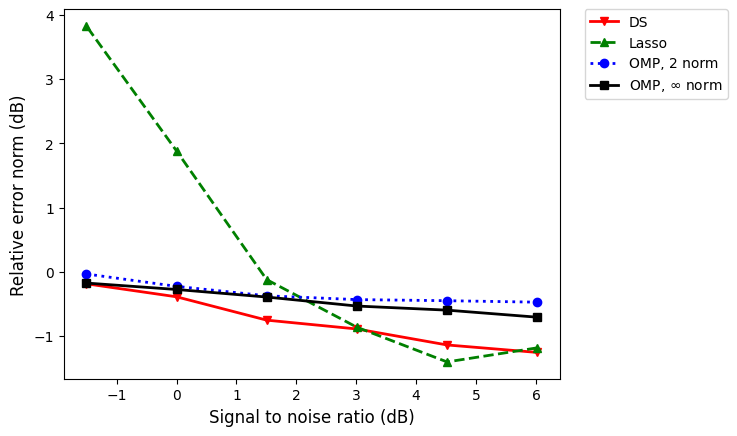
\includegraphics [width = 0.45 \textwidth]
{error-small-more-tall-six-usual.png}
\caption {\m {N_B = 2, N_{H,t} = 6, N_{H,r} = 8}, error.}
\end {figure}

\begin {figure} [H]
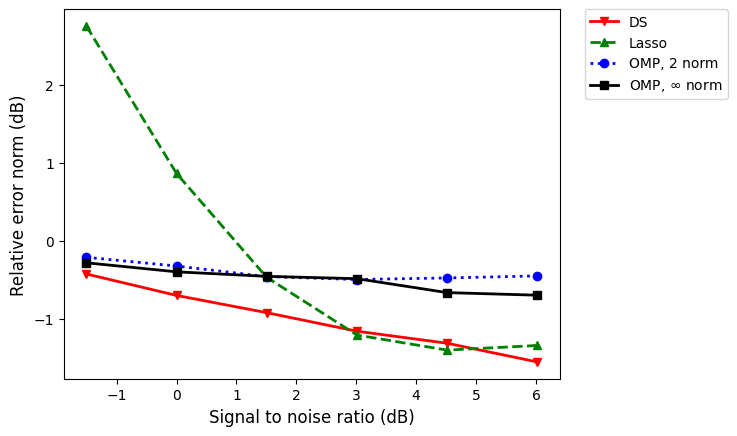
\includegraphics [width = 0.45 \textwidth]
{error-small-more-wide-six-usual.png}
\caption {\m {N_B = 2, N_{H,t} = 8, N_{H,r} = 6}, error.}
\end {figure}

\begin {figure} [H]
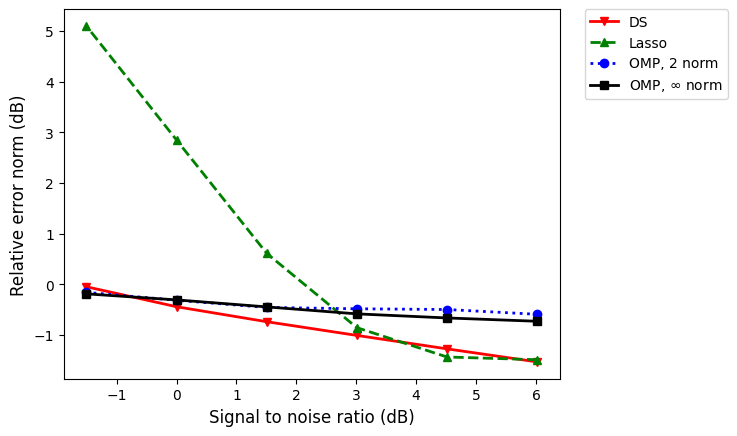
\includegraphics [width = 0.45 \textwidth]
{error-medium-more-tall-six-usual.png}
\caption {\m {N_B = 4, N_{H,t} = 12, N_{H,r} = 16}, error.}
\end {figure}

\begin {figure} [H]
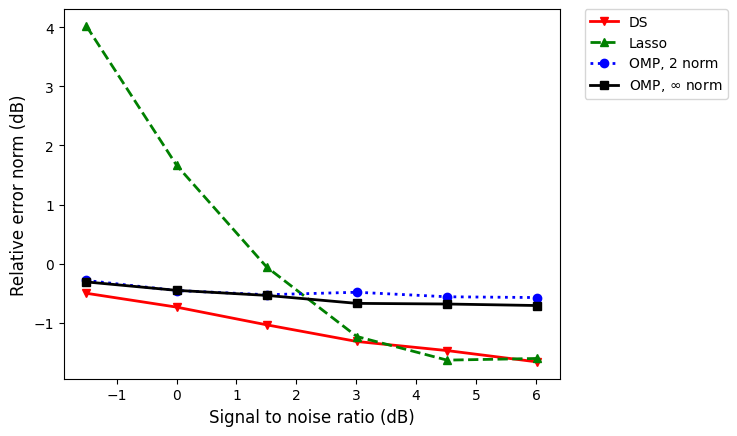
\includegraphics [width = 0.45 \textwidth]
{error-medium-more-wide-six-usual.png}
\caption {\m {N_B = 4, N_{H,t} = 16, N_{H,r} = 12}, error.}
\end {figure}

\begin {figure} [H]
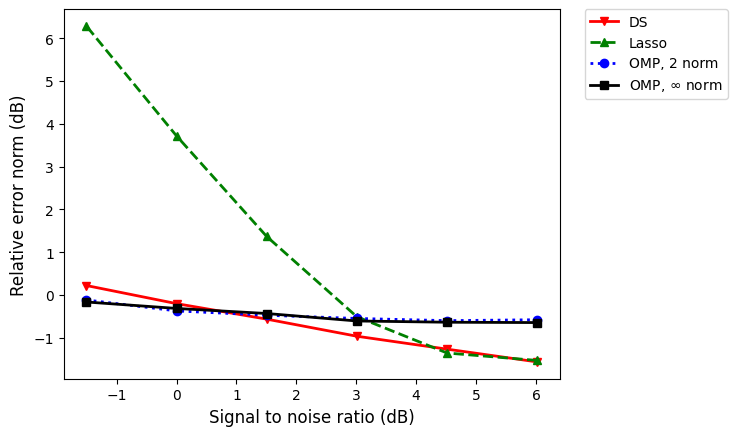
\includegraphics [width = 0.45 \textwidth]
{error-big-more-tall-six-usual.png}
\caption {\m {N_B = 6, N_{H,t} = 24, N_{H,r} = 18}, error.}
\end {figure}

\begin {figure} [H]
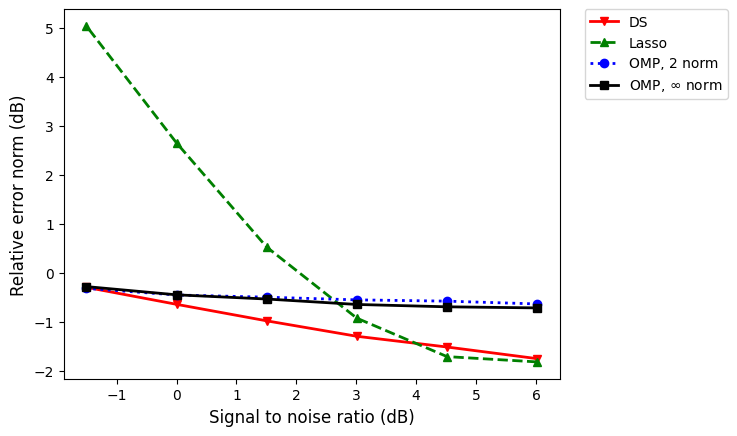
\includegraphics [width = 0.45 \textwidth]
{error-big-more-wide-six-usual.png}
\caption {\m {N_B = 6, N_{H,t} = 18, N_{H,r} = 24}, error.}
\end {figure}

\subsection {Discussion}

From the simulation, DS outperforms other methods in most of the datasets.
With low noise, \m {\tilde {\chi} _{\mathrm {DS}} \approx \tilde {\chi} _{\mathrm {OMP}} \leq \tilde {\chi} _{\mathrm {Lasso}} \leq \tilde {\chi} _{\mathrm {LS}}},
although sometimes \m {\tilde {\chi} _{\mathrm {DS}} \geq \tilde {\chi} _{\mathrm {OMP}}}.
With high noise, \m {\tilde {\chi} _{\mathrm {DS}} \approx \tilde {\chi} _{\mathrm {Lasso}} \leq \tilde {\chi} _{\mathrm {OMP}} \leq \tilde {\chi} _{\mathrm {LS}}}.
although sometimes \m {\tilde {\chi} _{\mathrm {DS}} \geq \tilde {\chi} _{\mathrm {Lasso}}}.
LS is so much poorer that it is not a main contender.
These trends is true with different number of stages, and with the case \m {N_B = N_R}.
In general, we can say that overall, DS gives a better regularization for both low noise and high noise scenario, and in most cases, DS is even better than both of them.

Differing thresholds does not to seem have much effect on OMP and DS.
Meanwhile for Lasso, where a suitable threshold may improve the accuracy, but a excessively tight threshold may also result in a overfitting, and blowing up for high signal cases.
Increasing the number of stages obviously improves the estimation for all methods.

Unfortunately, we report that CVXPY sometimes gives overflowing values, some of them as large as \m {10^{11}}.
This probably indicates some typical-looking output may in fact be unreliable.
Therefore we have discarded outputs larger than a given threshold, for instance \m {10^4}, and simply return the answer to be a Moore–Penrose inverse.

\m {\chi} is not shown in the figure, because the big O bound is much larger than \m {\tilde {\chi}}.
It is possible that the nonsparsity of \m {\V {g}} undermines the analysis in chapter 3, despite our attempts to account for that effect.
It is curious to see whether for very large \m {N_H}, whether \m {\tilde {\chi}} and \m {\chi} will be asymptotically close.

\subsection {Complexity}

We discuss the complexity of DS, Lasso, and OMP.
For DS, suppose a linear program has an \m {N} dimensional variable and \m {M} inequality constraints, then its complexity is \m {\mathcal {O} \SB {N^2 M}}, assuming the Dantzig simplex method is used \cite {BoV04}.
For our case, that would be \m {\mathcal {O} \SB {4 N_h ^2 \D 8 N_h} = \mathcal {O} \SB {N_h ^3}}.

Alternatively, suppose Newton method is used.
Here, we have self-concordance for linear program \cite {BoV04}.
Let \m {\V {g} _0} denote the starting value of \m {\V {g}'}, and \m {\V {g} ^{\star}} the the point of convergence.
Then the number of Newton steps, which we take to be the complexity, is bounded by \cite {BoV04}
\Disp {
C_{\mathrm {Newton}}
\propto \RB {\VNm {\V {g}_0 -\V {g} ^{\star}}_1
+ \log_2 \log_2 \frac {1} {\e}}
}

Assume that, at the start the iteration, the Moore–Penrose inverse is close to the initial value of \m {\V {g}_0}, namely
%
\Disp {
\V {g}_0
=\V {g}_{\mathrm {LS}}
= \RB {\M {P} ^\dagger \M {P}} ^{-1} \M {P} ^\dagger \V {y} 
}
And suppose that, in view of restricted isometry, \m {\M {P}} has unity-normed, almost orthogonal columns, so that
\m {\M {P} ^\dagger \M {P} \approx I _{N_h}}
Moreover, assume that \m {\V {g} ^\star \approx \V {g}}.
Then we simply have
\Disp {
C_{\mathrm {DS}}
=\mathcal {O} \SB {N_h ^3} 
}

For OMP \cite {TrG07}, \m {C_{\mathrm {OMP}} =\mathcal {O} \SB {L \RB {\log N_h} ^2}}.

For Lasso, it is equivalent to a quadratically constrained quadratic program, and there is not always a closed form for its complexity.
However, Lasso and DS are equivalent in certain conditions \cite {AsR10}, and we may suppose here they have the same complexity.
Alternatively, an argument similar to the above one for DS is valid for Lasso.
Therefore we take \m {C_{\mathrm {Lasso}} =\mathcal {O} \SB {N_h ^3}}.


% % % % % % % % % % % % % % % % % % % % % % % % % % % % % % % %
% % % % % % % % % % % % % % % % % % % % % % % % % % % % % % % %

\section{Conclusion}

The treatise aims to answer the problem of effective estimating a MIMO mm-wave channel by exploiting its sparsity.
To do so, we apply the Dantzig Selector (DS), by exploiting the sparsity in the spatial frequency domain, and justified the restricted isometry of the effective beamforming matrix.
We then prove quantitatively that the expected error norm is bounded for overwhelming probability.
We also suggest several ways of reducing the complexity without losing much performance.
Simulation is done, and we see that DS indeed outperforms other methods in most datasets.

Since we have RIP, a whole series of compressive sensing techniques become possible.
But moreover, we corroborate the prediction that DS gives better regularization, and it may extract more information than other methods do when the sampling rate is low.
In particular, when the sample is less abundant and the noise level is higher, sometimes only DS can recover successfully.
Therefore, one may use DS for sake of higher precision, or with limited RF chains and fewer stages of estimation, for example, in the ultra reliable or low latency scenario.

\section*{Acknowledgment}

The authors would like to thank the heaven.

% % % % % % % % % % % % % % % % % % % % % % % % % % % % % % % %
% % % % % % % % % % % % % % % % % % % % % % % % % % % % % % % %

\begin{thebibliography}{30}
\bibitem{RSM13}
T. S. Rappaport, S. Sun, R. Mayzus, H. Zhao, Y. Azar, K. Wang, G. N. Wong, J. K. Schulz, M. Samimi, and F. Gutierrez, “Millimeter wave mobile communications for 5g cellular: It will work!” \textit {IEEE access}, vol. 1, pp. 335–349, 2013.

\bibitem{RDD18}
M. Rani, S. B. Dhok, and R. Deshmukh, “A systematic review of compressive sensing: Concepts, implementations and applications,” \textit {IEEE Access}, vol. 6, pp. 4875–4894, 2018.

\bibitem{CaT05}
E. J. Candès and T. Tao, “Decoding by linear programming,” \textit {IEEE Transactions on Information Theory}, vol. 51, no. 12, p. 4203, 2005.

\bibitem{CaT07}
E. Candès and T. Tao, “The dantzig selector: Statistical estimation when p is much larger than n,” \textit {The annals of Statistics}, vol. 35, no. 6, pp. 2313–2351, 2007.

\bibitem{BDD08}
[6] R. Baraniuk, M. Davenport, R. DeVore, and M. Wakin, “A simple proof of the restricted isometry property for random matrices,” \textit {Constructive Approximation}, vol. 28, no. 3, pp. 253–263, 2008.

\bibitem{BHS10}
W. U. Bajwa, J. Haupt, A. M. Sayeed, and R. Nowak, “Compressed channel sensing: A new approach to estimating sparse multipath channels,” \textit {Proceedings of the IEEE}, vol. 98, no. 6, pp. 1058–1076, 2010.

\bibitem{BHR08}
W. U. Bajwa, J. Haupt, G. Raz, and R. Nowak, “Compressed channel sensing,” 2008 \textit {42nd Annual Conference on Information Sciences and Systems}, pp. 5–10, 2008.

\bibitem{AsR10}
M. S. Asif and J. Romberg, “On the lasso and dantzig selector equivalence,” 2010 \textit {44th Annual Conference on Information Sciences and Systems} (CISS), pp. 1–6, 2010.

\bibitem{LLL17}
L. Lian, A. Liu, and V. K. Lau, “Optimal-tuned weighted lasso for massive mimo channel estimation with limited rf chains,” \textit {IEEE Global Communications Conference}, pp. 1–6, 2017.

\bibitem{DJN15}
G. Destino, M. Juntti, and S. Nagaraj, “Leveraging sparsity into massive mimo channel estimation with the adaptive-lasso,” \textit {IEEE Global Conference on Signal and Information Processing} (GlobalSIP), pp. 166–170, 2015.

\bibitem{VAT19}
E. Vlachos, G. C. Alexandropoulos, and J. Thompson, “Wideband mimo channel estimation for hybrid beamforming millimeter wave systems via random spatial sampling,” \textit {IEEE Journal of Selected Topics in Signal Processing}, vol. 13, no. 5, pp. 1136–1150, 2019.

\bibitem{TrG07}
J. A. Tropp and A. C. Gilbert, “Signal recovery from random measurements via orthogonal matching pursuit,” \textit {IEEE Transactions on information theory}, vol. 53, no. 12, pp. 4655–4666, 2007.

\bibitem{ALH15}
A. Alkhateeb, G. Leus, and R. W. Heath, “Compressed sensing based multi-user millimeter wave systems: How many measurements are needed?” 2015 \textit {IEEE International Conference on Acoustics, Speech and Signal Processing} (ICASSP), pp. 2909–2913, 2015.

\bibitem{HWH13}
D. Hu, X. Wang, and L. He, “A new sparse channel estimation and tracking method for time-varying ofdm systems,” \textit {IEEE Transactions on Vehicular Technology}, vol. 62, no. 9, pp. 4648–4653, 2013.

\bibitem{LGL16}
J. Lee, G.-T. Gil, and Y. H. Lee, “Channel estimation via orthogonal matching pursuit for hybrid mimo systems in millimeter wave communications,” \textit {IEEE Transactions on Communications}, vol. 64, no. 6, pp. 2370–2386, 2016.

\bibitem{GDW15}
Z. Gao, L. Dai, Z. Wang, and S. Chen, “Spatially common sparsity based adaptive channel estimation and feedback for fdd massive mimo,” \textit {IEEE Transactions on Signal Processing}, vol. 63, no. 23, pp. 6169–6183, 2015.

\bibitem{CWX10}
T. T. Cai, L. Wang, and G. Xu, “Stable recovery of sparse signals and an oracle inequality,” \textit {IEEE Transactions on Information Theory}, vol. 56, no. 7, pp. 3516–3522, 2010.

\bibitem{CaW11}
T. T. Cai and L. Wang, “Orthogonal matching pursuit for sparse signal recovery with noise,” \textit {IEEE Transactions on Information Theory}, 2011.

\bibitem{BEE10}
Z. Ben-Haim, Y. C. Eldar, and M. Elad, “Coherence-based performance guarantees for estimating a sparse vector under random noise,” \textit {IEEE Transactions on Signal Processing}, vol. 58, no. 10, pp. 5030–5043, 2010.

\bibitem{ALS14}
M. R. Akdeniz, Y. Liu, M. K. Samimi, S. Sun, S. Rangan, T. S. Rappaport, and E. Erkip, “Millimeter wave channel modeling and cellular capacity evaluation,” \textit {IEEE journal on selected areas in communications}, vol. 32, no. 6, pp. 1164–1179, 2014.

\bibitem{LaM00}
B. Laurent and P. Massart, “Adaptive estimation of a quadratic functional by model selection,” \textit {Annals of Statistics}, pp. 1302–1338, 2000.

\bibitem{KlM17}
B. Klartag and E. Milman, \textit {Geometric Aspects of Functional Analysis}. Springer, 2017.

\bibitem{BoV04}
S. Boyd and L. Vandenberghe, \textit {Convex optimization}. Cambridge U. press, 2004.

\bibitem{FrS07}
M. P. Friedlander and M. A. Saunders, “Discussion: The dantzig selector: Statistical estimation when p is much larger than n,” \textit {The Annals of Statistics}, vol. 35, no. 6, pp. 2385–2391, 2007.

\end{thebibliography}


\end{document}


